\chapter{DAuth: The Base Authentication Scheme}

\section{Overview of DAuth}

DAuth~\cite{das2026comsnets} is designed for multihop IoT networks where
newly joined nodes must authenticate themselves securely before communicating with
the gateway.
Instead of relying on a centralised authority, the gateway distributes the
authentication workload by selecting a set of already-authenticated IoT nodes to
operate as Authentication Servers (AS).
Let this set be represented as $\mathcal{AS}' = \{AS_1, AS_2, \ldots, AS_n\}$,
where the gateway shares a long-term secret key $K_{GW\text{-}AS}$ with each $AS_i$.

When a new device $D$ joins the network, the gateway (through the parent node)
provides $D$ with the address and identity $ID_{AS}$ of the responsible
authenticator.
Importantly, the AS may lie at a single-hop or multi-hop distance, and does not need
to be the parent node.
This \emph{decoupling} reduces the computational burden on both gateway and parent
nodes, improving scalability in dense IoT environments.

The operation of the scheme is divided into two major phases: the
\textbf{Node Enrollment Phase} and the \textbf{Node Authentication and Key Exchange
Phase}.

\subsection{Node Enrollment Phase}

In the enrollment phase, node $D$ communicates with its AS over a secure channel.
During enrollment, $D$ generates its unique secret $y_D$, hashes it to obtain
$Y_D = H(y_D)$, and registers this value with the AS.
The AS incorporates $Y_D$ into its hash-based accumulator using
$T_{\mathsf{Acc}} = T_{\mathsf{Acc}}\ \&\ Y_D$.
To avoid storing large CRP databases, the AS stores only a lightweight entry
consisting of the challenge $c_{AS\text{-}D}$ and a masked PUF response
$\Phi_D = R_{AS\text{-}D} \oplus R_D$, while $D$ stores its own challenge $c_D$.
This significantly reduces memory usage and prevents direct leakage of raw PUF
responses.
Figure~\ref{fig:base_enroll} illustrates this phase.

\begin{figure}[!ht]
  \centering
  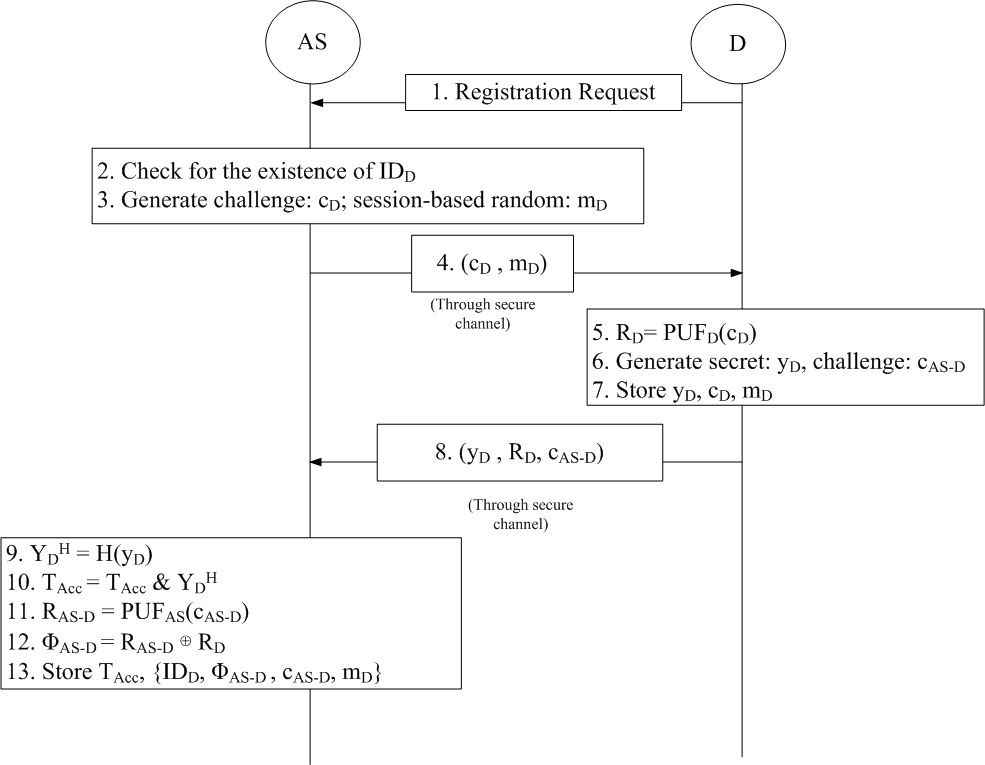
\includegraphics[width=0.82\textwidth]{EnrollmentPhase}
  \caption{Node Enrollment Phase of DAuth (adapted from~\cite{das2026comsnets}).}
  \label{fig:base_enroll}
\end{figure}

\subsection{Node Authentication and Key Exchange Phase}

In the \textbf{Node Authentication Phase}, node $D$ authenticates itself to the AS
over an insecure public channel.
$D$ regenerates its PUF response $R_D = \mathsf{PUF}_D(c_D)$ and computes a mask
$H(R_D \| m_D \| ID_D \| ts_1)$, where $m_D$ is the current session-based random
obtained during enrollment.
The hashed witness $Y_D^H = H(y_D)$ is XORed with this mask and transmitted to the
AS along with the real device identity $ID_D$ and timestamp $ts_1$.

Upon receiving the message, AS reconstructs $R_D$ using $\Phi_D \oplus R_{AS\text{-}D}$,
regenerates the mask, unmasks $Y_D^{H'}$, and verifies authenticity by checking
$T_{\mathsf{Acc}}\ \&\ Y_D^{H'} = T_{\mathsf{Acc}}$.
If equality holds, the AS confirms that $D$ was previously registered.
Figure~\ref{fig:base_auth} shows the authentication phase.

\begin{figure}[!ht]
  \centering
  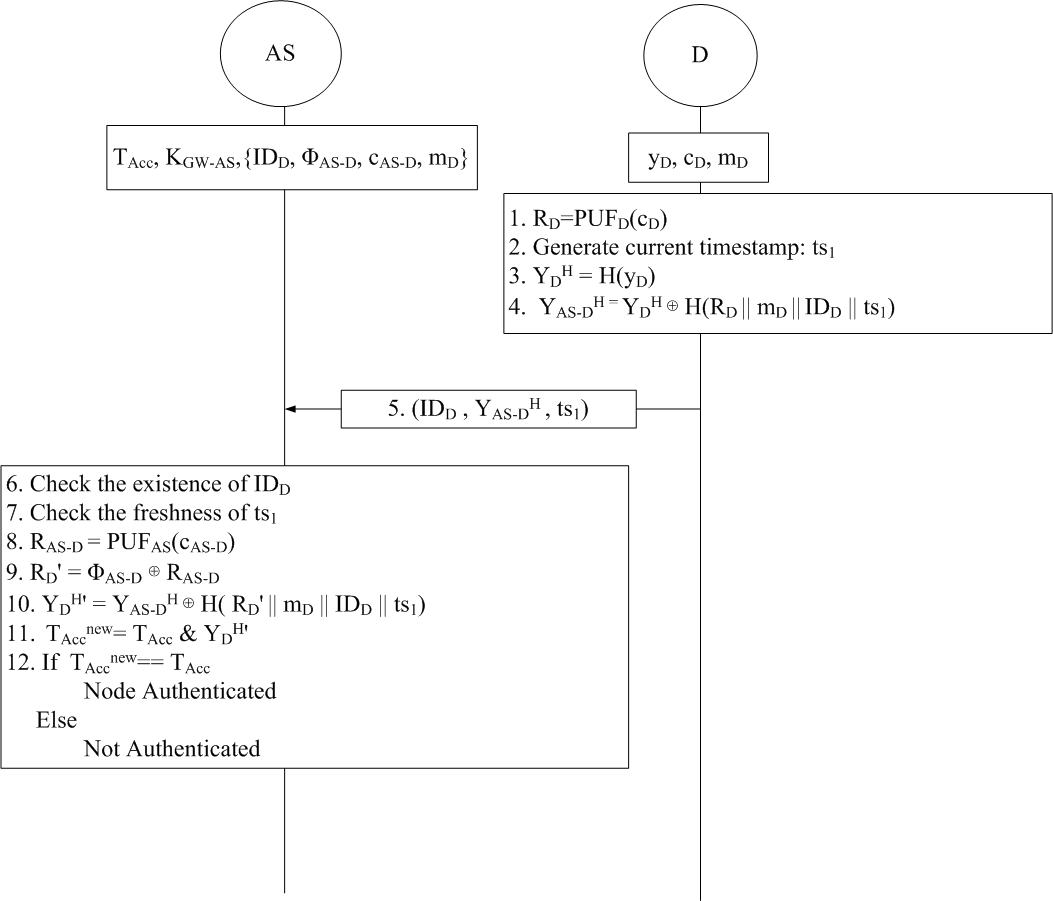
\includegraphics[width=0.82\textwidth]{AuthenticationPhase}
  \caption{Node Authentication Phase of DAuth (adapted from~\cite{das2026comsnets}).}
  \label{fig:base_auth}
\end{figure}

The AS then generates a new session-based random $m_{\mathrm{new}} = H(n_1)$, where
$n_1$ is freshly chosen, replacing $m_D$ for the next session and providing forward
secrecy.
The session key for secure communication between the gateway and the node is computed
as $K_{GW\text{-}D} = H(R_D \| m_{\mathrm{new}})$.
AS constructs an authentication token containing $ID_D$, $ID_{AS}$, timestamp
$ts_{\mathrm{auth}}$, and the session key $K_{GW\text{-}D}$, encrypted under
$K_{GW\text{-}AS}$, and sends it to the gateway.
Figure~\ref{fig:base_keyex} illustrates this key exchange.

\begin{figure}[!ht]
  \centering
  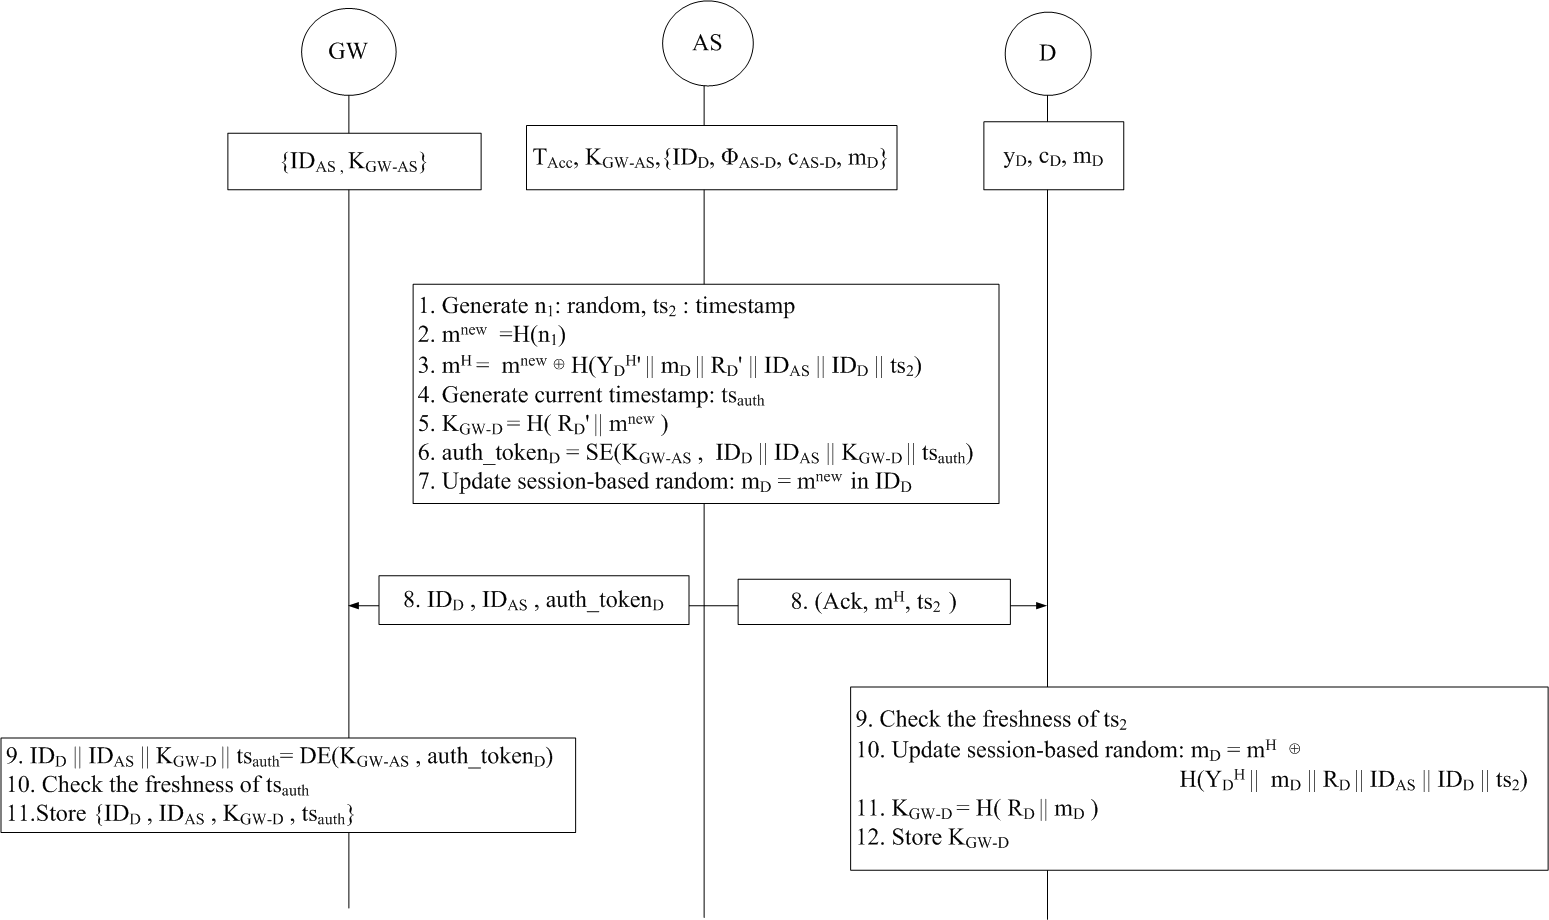
\includegraphics[width=0.95\textwidth]{KeyExchange}
  \caption{Node Key Exchange Phase of DAuth (adapted from~\cite{das2026comsnets}).}
  \label{fig:base_keyex}
\end{figure}

\subsection{Privacy Gaps in DAuth}

Although DAuth achieves decoupled and distributed authentication,
PUF-based security, lightweight computation, low storage overhead, and dynamic key
updates, it leaves two critical gaps unaddressed.

\textbf{Gap 1: Identity Exposure}
The real device identity $ID_D$ is transmitted in plaintext on the open channel in
every authentication session.
In the open wireless environments typical of IoT deployments, a passive attacker
monitoring the channel can readily capture these identity transmissions.
Even when all other packet fields carry opaque values, the presence of a plaintext
$ID_D$ is sufficient for an adversary to link multiple authentication attempts to
the same device.
Accumulated over time, such captures enable long-term device tracking, session
linkage, topology inference, and targeted denial-of-service against specific nodes.
In a multihop network, the exposure is amplified, since each intermediate hop
introduces an additional vantage point from which the identity can be observed.

\textbf{Gap 2: Desynchronisation}
DAuth stores only a single session nonce $m_D$ at the AS.
If the key-exchange response carrying the new $m_{\mathrm{new}}$ to device $D$ is
lost, $D$ retains the old $m_D$ while the AS has already advanced to $m_{\mathrm{new}}$.
On the next authentication attempt, $D$ constructs its authentication message using
the stale $m_D$, but the AS uses $m_{\mathrm{new}}$ to verify; the masks no longer
match, authentication fails, and the device must undergo full re-enrolment.

These two deficiencies motivate the proposed scheme, which hides device identities
from the open channel, prevents session linkage, and adds desynchronisation
resilience while preserving the lightweight and distributed character of DAuth.
